\documentclass{article}

%%%%%%%%%%%%%%%%%%%%%%%%%%%%%%%%%%%%%%%%%
% Lachaise Assignment
% Structure Specification File
% Version 1.0 (26/6/2018)
%
% This template originates from:
% http://www.LaTeXTemplates.com
%
% Authors:
% Marion Lachaise & François Févotte
% Vel (vel@LaTeXTemplates.com)
%
% License:
% CC BY-NC-SA 3.0 (http://creativecommons.org/licenses/by-nc-sa/3.0/)
% 
%%%%%%%%%%%%%%%%%%%%%%%%%%%%%%%%%%%%%%%%%

%----------------------------------------------------------------------------------------
%	PACKAGES AND OTHER DOCUMENT CONFIGURATIONS
%----------------------------------------------------------------------------------------

\usepackage{amsmath,amsfonts,stmaryrd,amssymb} % Math packages

\usepackage{enumerate} % Custom item numbers for enumerations

\usepackage[ruled]{algorithm2e} % Algorithms

\usepackage[framemethod=tikz]{mdframed} % Allows defining custom boxed/framed environments

\usepackage{listings} % File listings, with syntax highlighting
\lstset{
	basicstyle=\ttfamily, % Typeset listings in monospace font
}

%----------------------------------------------------------------------------------------
%	DOCUMENT MARGINS
%----------------------------------------------------------------------------------------

\usepackage{geometry} % Required for adjusting page dimensions and margins

\geometry{
	paper=a4paper, % Paper size, change to letterpaper for US letter size
	top=2.5cm, % Top margin
	bottom=3cm, % Bottom margin
	left=2.5cm, % Left margin
	right=2.5cm, % Right margin
	headheight=14pt, % Header height
	footskip=1.5cm, % Space from the bottom margin to the baseline of the footer
	headsep=1.2cm, % Space from the top margin to the baseline of the header
	%showframe, % Uncomment to show how the type block is set on the page
}

%----------------------------------------------------------------------------------------
%	FONTS
%----------------------------------------------------------------------------------------

\usepackage[utf8]{inputenc} % Required for inputting international characters
\usepackage[T1]{fontenc} % Output font encoding for international characters

\usepackage{XCharter} % Use the XCharter fonts

%----------------------------------------------------------------------------------------
%	COMMAND LINE ENVIRONMENT
%----------------------------------------------------------------------------------------

% Usage:
% \begin{commandline}
%	\begin{verbatim}
%		$ ls
%		
%		Applications	Desktop	...
%	\end{verbatim}
% \end{commandline}

\mdfdefinestyle{commandline}{
	leftmargin=10pt,
	rightmargin=10pt,
	innerleftmargin=15pt,
	middlelinecolor=black!50!white,
	middlelinewidth=2pt,
	frametitlerule=false,
	backgroundcolor=black!5!white,
	frametitle={Command Line},
	frametitlefont={\normalfont\sffamily\color{white}\hspace{-1em}},
	frametitlebackgroundcolor=black!50!white,
	nobreak,
}

% Define a custom environment for command-line snapshots
\newenvironment{commandline}{
	\medskip
	\begin{mdframed}[style=commandline]
}{
	\end{mdframed}
	\medskip
}

%----------------------------------------------------------------------------------------
%	FILE CONTENTS ENVIRONMENT
%----------------------------------------------------------------------------------------

% Usage:
% \begin{file}[optional filename, defaults to "File"]
%	File contents, for example, with a listings environment
% \end{file}

\mdfdefinestyle{file}{
	innertopmargin=1.6\baselineskip,
	innerbottommargin=0.8\baselineskip,
	topline=false, bottomline=false,
	leftline=false, rightline=false,
	leftmargin=2cm,
	rightmargin=2cm,
	singleextra={%
		\draw[fill=black!10!white](P)++(0,-1.2em)rectangle(P-|O);
		\node[anchor=north west]
		at(P-|O){\ttfamily\mdfilename};
		%
		\def\l{3em}
		\draw(O-|P)++(-\l,0)--++(\l,\l)--(P)--(P-|O)--(O)--cycle;
		\draw(O-|P)++(-\l,0)--++(0,\l)--++(\l,0);
	},
	nobreak,
}

% Define a custom environment for file contents
\newenvironment{file}[1][File]{ % Set the default filename to "File"
	\medskip
	\newcommand{\mdfilename}{#1}
	\begin{mdframed}[style=file]
}{
	\end{mdframed}
	\medskip
}

%----------------------------------------------------------------------------------------
%	NUMBERED QUESTIONS ENVIRONMENT
%----------------------------------------------------------------------------------------

% Usage:
% \begin{question}[optional title]
%	Question contents
% \end{question}

\mdfdefinestyle{question}{
	innertopmargin=1.2\baselineskip,
	innerbottommargin=0.8\baselineskip,
	roundcorner=5pt,
	nobreak,
	singleextra={%
		\draw(P-|O)node[xshift=1em,anchor=west,fill=white,draw,rounded corners=5pt]{%
		Question \theQuestion\questionTitle};
	},
}

\newcounter{Question} % Stores the current question number that gets iterated with each new question

% Define a custom environment for numbered questions
\newenvironment{question}[1][\unskip]{
	\bigskip
	\stepcounter{Question}
	\newcommand{\questionTitle}{~#1}
	\begin{mdframed}[style=question]
}{
	\end{mdframed}
	\medskip
}

%----------------------------------------------------------------------------------------
%	WARNING TEXT ENVIRONMENT
%----------------------------------------------------------------------------------------

% Usage:
% \begin{warn}[optional title, defaults to "Warning:"]
%	Contents
% \end{warn}

\mdfdefinestyle{warning}{
	topline=false, bottomline=false,
	leftline=false, rightline=false,
	nobreak,
	singleextra={%
		\draw(P-|O)++(-0.5em,0)node(tmp1){};
		\draw(P-|O)++(0.5em,0)node(tmp2){};
		\fill[black,rotate around={45:(P-|O)}](tmp1)rectangle(tmp2);
		\node at(P-|O){\color{white}\scriptsize\bf !};
		\draw[very thick](P-|O)++(0,-1em)--(O);%--(O-|P);
	}
}

% Define a custom environment for warning text
\newenvironment{warn}[1][Warning:]{ % Set the default warning to "Warning:"
	\medskip
	\begin{mdframed}[style=warning]
		\noindent{\textbf{#1}}
}{
	\end{mdframed}
}

%----------------------------------------------------------------------------------------
%	INFORMATION ENVIRONMENT
%----------------------------------------------------------------------------------------

% Usage:
% \begin{info}[optional title, defaults to "Info:"]
% 	contents
% 	\end{info}

\mdfdefinestyle{info}{%
	topline=false, bottomline=false,
	leftline=false, rightline=false,
	nobreak,
	singleextra={%
		\fill[black](P-|O)circle[radius=0.4em];
		\node at(P-|O){\color{white}\scriptsize\bf i};
		\draw[very thick](P-|O)++(0,-0.8em)--(O);%--(O-|P);
	}
}

% Define a custom environment for information
\newenvironment{info}[1][Info:]{ % Set the default title to "Info:"
	\medskip
	\begin{mdframed}[style=info]
		\noindent{\textbf{#1}}
}{
	\end{mdframed}
}


 % Include the file specifying the document structure and custom commands


%----------------------------------------------------------------------------------------
%	ASSIGNMENT INFORMATION
%----------------------------------------------------------------------------------------

\title{Problem Set \#1} % Title of the assignment

\author{Saharnaz Babaei Balderlou\\ \texttt{saharnaz.babaei@grad.moore.sc.edu}} % Author name and email address

\date{University of South Carolina --- \today} % University, school and/or department name(s) and a date

%----------------------------------------------------------------------------------------

\begin{document}

\maketitle % Print the title

%----------------------------------------------------------------------------------------
%	INTRODUCTION
%----------------------------------------------------------------------------------------

\section*{Introduction} % Unnumbered section
Last decade started with a devastating economic downturn, the big credit crisis in 2007-2008. This crisis was the result of a set of complicated and risky policies in the US financial and housing markets but very quickly spread in the world and covered much of the world as the flames of a wildfire. This crisis showed how an economic fluctuation can burn the other parts of society and stunt them. It can even affect in the individual level and devastate people’s lives.\\
A broad definition of economic crisis is composed of different kinds of crises such as public finance crisis, interest rate and sheet of balance related crisis. There are so many reasons for starting and origination of economic and financial crises; expansionary policies and budget deficit which can contribute to bubbles in the economy, imbalances of balance sheet, inappropriate inflation targeting towards the inflation in anchor currency country, expectations and speculative attacks (\cite{billio2005multivariate}). \\
Some crises occur in a country and affect only that economy. But sometimes, crisis occurred in an economy is outspread to other economies. This latter situation is known as contagion effect. In economics, contagion effect is considered as a local, national or regional situation in which a shock in an economy moves to and effects on another one in a sense of price movement. We define contagion broadly not only as the negative transmission of shocks, but also any shock occurred in one country with a spillover effect in another economy or country. \\
Some of the above-mentioned reasons of crisis seem to be internal to an economy but in fact, we can see that in a globalized world, they are connected. For example, as we have seen in the follow up of the 2007-2008 crisis, economic policies are not anymore apart from each other in several countries which are interconnected due to the presence of large international organizations. Globalization also increases this interconnection in the sense of political and economic terms by making the economies to be closer and deeper integrated.  \\
Globalization is a multidimensional phenomenon that eliminates the economic, political, and cultural borders, leads to changes in trade and transaction rules, dissemination of knowledge and technology, and migration and movement of people. Eventually it can result in an integration of the countries by creating a global market-place or a single world market. After WW II, cross-border flow of goods, services, capital, technology and information provided a ground for contagion effect. Hence, higher interdependency between economies has increased the flow of shocks. \\
On the other hand, globalization increases openness of a country, reduces barriers to trade, eliminates tariffs and increases international competition. In fact, improved macroeconomic performance and the ground for sharing risks are the benefits of financial globalization \cite{kose2009does}. Financial globalization is a starting point and source of crisis by causing imbalances in the credit market and current account. But regardless of this origination effect of globalization on crisis, it leads to a lower capital flow by increased global risk because the investors would prefer to not make international commitments and seek to leave their position with high risk environment (\cite{forbes2012capital, lane2013financial}). On the other hand, some characteristics of the capital flow could be the other edge of the sword and have a stabilizing force. For instance, some foreign investors may seek a bargain and invest on the domestic asset with reduced prices during the crises (\cite{lane2013financial}). Also, repatriation of the foreign assets may help the recovery of a domestic crises.  \\ 
With excess capital gains and losses on the foreign assets and liabilities, the international investment position is improved which can be considered as another stabilizing force during the crisis period. However, valuation losses play an important role as a crisis amplifier. In fact, exchange rate depreciation along with foreign currency debt lead to negative valuation effects that exacerbates crises effects.  \\
Looking at the 2008 crisis, foreign investors from advanced economies invested in asset-backed securities; while the investors from emerging markets invested in government-backed securities and decreased their risk of being exposed to the crisis (\cite{lane2013financial}).  \\
To better understand the relation between globalization and contagion effect, we need to recognize the channels through which the shocks transmit between economies. In fact, there are trade linkages and financial linkages among them. The first one relates to the regional and global trade integration and the latter is mainly related to the globalization of capital flows. Also, any policy in the domestic system can resist sudden and strong outflow and inflow of investment. Another protecting factor against crisis connected to the globalization is attempting to avoid crisis by interest rate policy (omitting any motivation to speculate with currency), international reserve usage and influencing investors’ expectations. By and large, globalization can be considered as both a factor of propagation of crisis and prevention of its occurrence in high volume. Hence, this study intends to assess the relationship between globalization and the propagation of the crises. \\
\section*{Methodology and data}
\subsection*{Markov-Switching panel specification} 
We are going to use the following baseline model to define the effects of globalization on contagion effect:
% Math equation/formula
\begin{equation}
\label{eq1}
con_{it} = D_{i} C_{i} + \sum_{k=1}^K \beta_{k} x_{kit} + \varepsilon_{it}
\end{equation}
Assume we have sample observations $K(k =1, …, K)$ features for $N(i =1, …, N)$ individuals and $T(t = 1, …, T)$ time periods. Let 
$$
\operatorname{con}_{i}=\left[\begin{array}{c}{y_{i 1}} \\ {\vdots} \\ {y_{i T}}\end{array}\right] ; \quad X_{i}=\left[\begin{array}{ccc}{X_{1 i 1}} & {\dots} & {X_{K i 1}} \\ {\vdots} & {\vdots} & {\vdots} \\ {X_{1 i T}} & {\dots} & {X_{K i T}}\end{array}\right]
$$
$$
j_{T}=\left[\begin{array}{l}{1} \\ {\vdots} \\ {1}\end{array}\right] ; \quad D=\left[\begin{array}{lll}{d_{1}} & {\ldots} & {d_{N}}\end{array}\right]=\left[\begin{array}{cccc}{j_{T}} & {0} & {\ldots} & {0} \\ {0} & {j_{T}} & {\ldots} & {\vdots} \\ {\vdots} & {\vdots} & {\vdots} & {0} \\ {0} & {\ldots} & {0} & {j_{T}}\end{array}\right] ; \quad \varepsilon_{i}=\left[\begin{array}{c}{\varepsilon_{i 1}} \\ {\varepsilon_{i 2}} \\ {\vdots} \\ {\varepsilon_{i T}}\end{array}\right]
$$

where $con_{i}$, $jT$ and $\varepsilon_{iT}$ are $T \times 1$ vectors and $X_{i}$ is a $T \times K$ matrix. Then we can rewrite equation (\ref{eq1}) as follows where $\beta$ is a $K \times 1$ vector:  
\begin{equation}
CON = Dc + X\beta + \varepsilon
\label{eq2}
\end{equation}
Equation \ref{eq2} is so-called least square dummy variable (LSDV) model and a Markov-Switching specification of panel model (MS-LSDV) is defined as follows: 
\begin{equation}
\operatorname{con}=D c(S_{t})+X \beta(S_{t})+\varepsilon(S_{t})
\label{eq3}
\end{equation}
where $\varepsilon(S_{t}) \sim N(0, \sigma^{2}(S_{t}))$ and $S_{t}$ is the state variable defined as a first order Markov chain:  
\begin{equation}
G=\left[\begin{array}{ll}{\operatorname{prob}\left(S_{t}=1 | S_{t-1}=1\right)} & {\operatorname{prob}\left(S_{t}=1 | S_{t-1}=2\right)} \\ {\operatorname{prob}\left(S_{t}=2 | S_{t-1}=1\right)} & {\operatorname{prob}\left(S_{t}=2 | S_{t-1}=2\right)}\end{array}\right]
\label{eq4}
\end{equation}
where $\operatorname{prob}\left(S_{t}=j | S_{t-1}=j^{\prime}\right)$ provides the probability of state $j$ if the state in the last period has been $j^{\prime}$ (either equal to $j$ or not). We consider an unobserved latent variable $S_{t}$ which takes value 1 when the economic state is tranquil (contagion is near 0) and 2 when it is frenzy (contagion is high). We do not discuss the algorithm of the Markov-Switching model here as it has been well documented in the extant literature(\cite{hansen1992likelihood,hansen1996erratum,quandt1972new,goldfeld1973markov}).  
\subsection*{Data} 
Different measurements are introduced in the literature for the contagion effect, including probability analysis, cross market correlation, VAR models, latent factor/Garch models and extreme values which is going to be used in this study. It is also called as co-exceedance or jump approach and is based on the first approach of probability analysis. In the extreme value analysis, the extreme moments are periods when realizations of certain variables exceed a large threshold value – with different approaches used to define these exceedances (\cite{forbes2012big}). In this study, both large increases and large decreases of both inflow and outflow of capital (following \cite{forbes2012capital}) is going to be considered. 
\begin{figure}
	\centering
	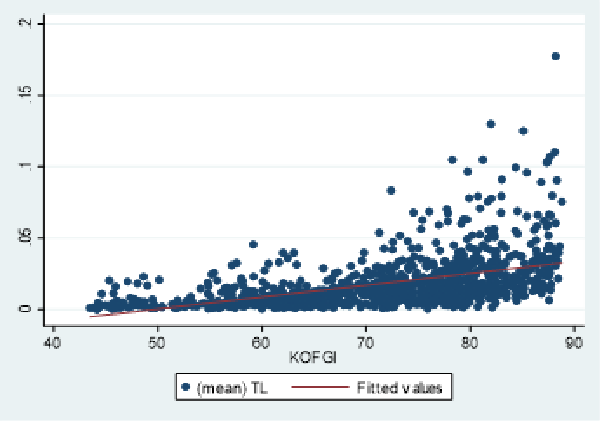
\includegraphics[width=10cm]{fig1.png}
	\caption{Scatter plot of contagion effect (trade linkages) versus globalization index }
	\label{fig:1}
\end{figure}
%----------------------------------------------------------------------------------------
\bibliographystyle{authordate1}
\bibliography{Ref}

\end{document}
